% IPMI Figure 3

\begin{figure}
\centering
\begin{tabular}{c c c c}
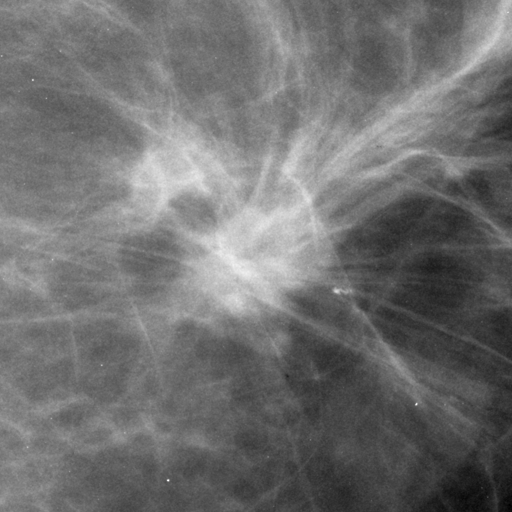
\includegraphics[width=\qtrcol]{\figpath/ipmi/mass028} &
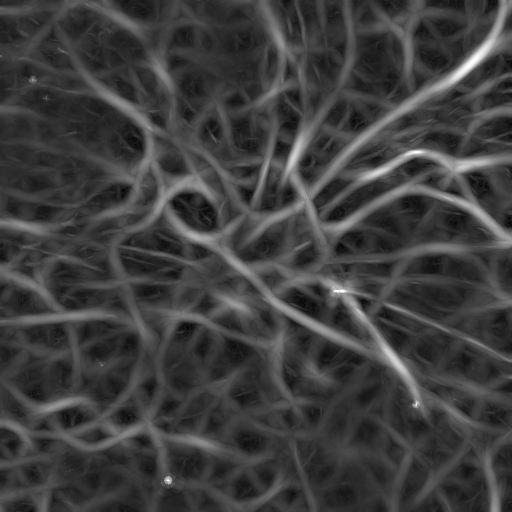
\includegraphics[width=\qtrcol]{\figpath/ipmi/mass028_linop} &
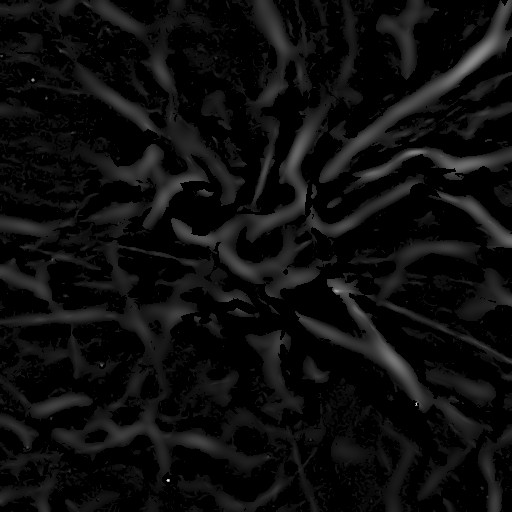
\includegraphics[width=\qtrcol]{\figpath/ipmi/mass028_gaussian} &
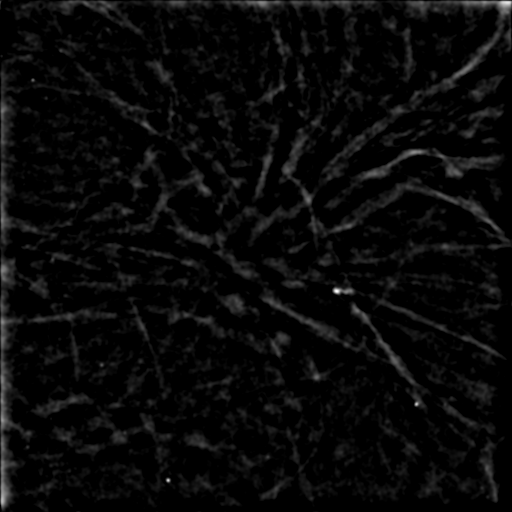
\includegraphics[width=\qtrcol]{\figpath/ipmi/mass028_monogenic} \\
(a) & (b) & (c) & (d) \\
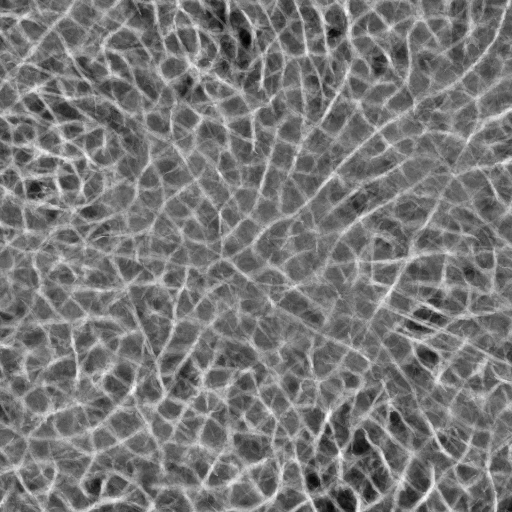
\includegraphics[width=\qtrcol]{\figpath/ipmi/mass028_dt} &
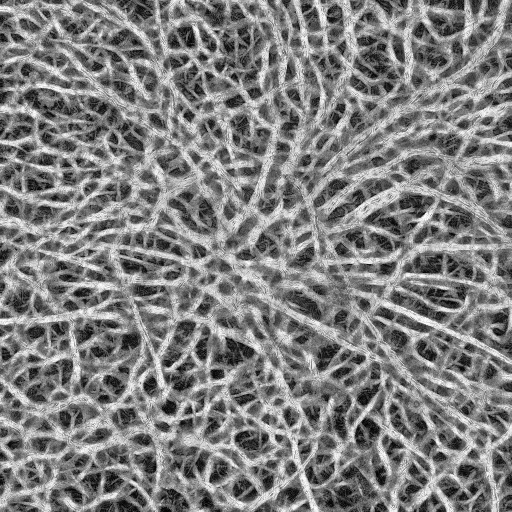
\includegraphics[width=\qtrcol]{\figpath/ipmi/mass028_rf_linop_w1l5} &
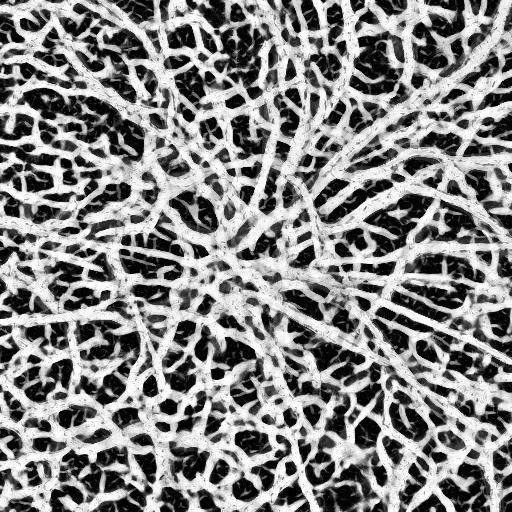
\includegraphics[width=\qtrcol]{\figpath/ipmi/mass028_rf_gaussian} &
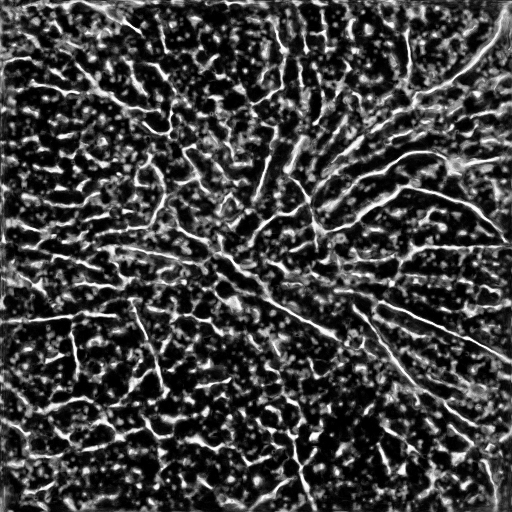
\includegraphics[width=\qtrcol]{\figpath/ipmi/mass028_rf_monogenic_w3l4} \\
(e) & (f) & (g) & (h)
\end{tabular}
%
\caption{Mammogram region containing malignant spiculated mass and corresponding filter responses: (a) original image; (b) Linop; (c) Gaussian; (d) Monogenic; (e) DT-CWT/RF; (f) Linop/RF; (g) Gaussian/RF; (h) Monogenic/RF.}
\label{f:real_responses}
\end{figure}